\section{The Elements of tkz code}

To work with my package, you need to have notions of \LATEX\ as well as \TIKZ.

In this paragraph, we start looking at the \code{rules} and \code{symbols} used to create a figure with \tkzname{\tkznameofpack}.

\subsection{Objects and language}

 The primitive objects are points. You can refer to a point at any time using the name given when defining it. (it is possible to assign a different name later on).

To get new points you will use macros. \tkzname{\tkznameofpack} macros have a name beginning with tkz. There are four main categories starting with:
|\tkzDef...| |\tkzDraw...| |\tkzMark...| and |\tkzLabel...|. 
The used points are passed as parameters between parentheses while the created points are between braces.

The code of the figures is placed in an environment \tkzimp{tikzpicture}


Contrary to \TIKZ, you should not end a macro with  “;”. We thus lose the important notion which is the \tkzimp{path}. However, it is possible to place some code between the macros \tkzname{\tkznameofpack}.
 

Among the first category, |\tkzDefPoint| allows you to define fixed points. It will be studied in detail later. Here we will see in detail the macro  |\tkzDefTriangle|.

This macro makes it possible to associate to a pair of points a third point in order to define a certain triangle |\tkzDefTriangle(A,B)|. The obtained point is referenced |tkzPointResult| and it is possible to choose another reference with |\tkzGetPoint{C}| for example.

|\tkzDefTriangle[euclid](A,B) \tkzGetPoint{C}|

Parentheses are used to pass arguments. In |(A,B)| $A$ and $B$ are the points with which a third will be defined. However, in |{C}| we use braces to retrieve the new point.

In order to choose a certain type of triangle among the following choices:
  |equilateral|,  |isosceles right|, |half|, |pythagoras|, |school|, |golden or sublime|, |euclid|, |gold|, |cheops|...
 and |two angles| you just have to choose between hooks, for example:
 
\begin{minipage}{0.5\textwidth}
  \begin{tikzpicture}[scale=.5]
  \tkzDefPoints{0/0/A,8/0/B}
  \foreach \tr in {golden, equilateral}
  {\tkzDefTriangle[\tr](A,B) \tkzGetPoint{C}
  \tkzDrawPoint(C)
  \tkzLabelPoint[right](C){\tr}
  \tkzDrawSegments(A,C C,B)}
  \tkzDrawPoints(A,B)
  \tkzDrawSegments(A,B)
   \tkzLabelPoints(A,B)
  \end{tikzpicture}
\end{minipage}
\begin{minipage}{0.5\textwidth}
  \begin{tkzexample}[code only,small]
    \begin{tikzpicture}[scale=.5]
    \tkzDefPoints{0/0/A,8/0/B}
   \foreach \tr in {golden, equilateral}
    {\tkzDefTriangle[\tr](A,B) \tkzGetPoint{C}
    \tkzDrawPoint(C)
    \tkzLabelPoint[right](C){\tr}
    \tkzDrawSegments(A,C C,B)}
    \tkzDrawPoints(A,B)
    \tkzDrawSegments(A,B)
    \tkzLabelPoints(A,B)
    \end{tikzpicture}
  \end{tkzexample}
\end{minipage}

\subsection{Notations and conventions}

I deliberately chose to use the geometric French and personal  conventions  to describe the geometric objects represented. The objects defined and represented by \tkzname{\tkznameofpack} are points, lines and circles located in a plane. They are the primary objects of Euclidean geometry from which we will construct figures.

According to \tkzimp{Euclid}, these figures will only illustrate pure ideas produced by our brain.
Thus a point has no dimension and therefore no real existence. In the same way the line has no width and therefore no existence in the real world. The objects that we are going to consider are only representations of ideal mathematical objects. \tkzname{\tkznameofpack} will follow the steps of the ancient Greeks to obtain geometrical constructions using the ruler and the compass. 

Here are the notations that will be used:

\begin{itemize}
\item The points are represented geometrically either by a small disc or by the intersection of two lines (two straight lines, a straight line and a circle or two circles). In this case, the point is represented by a cross. 

\begin{tkzexample}[latex=6cm, small]     
  \begin{tikzpicture}       
    \tkzDefPoints{0/0/A,4/2/B}       
    \tkzDrawPoints(A,B)       
    \tkzLabelPoints(A,B)     
  \end{tikzpicture}    
\end{tkzexample}

or else

\begin{tkzexample}[latex=6cm, small]     
  \begin{tikzpicture}       
    \tkzSetUpPoint[shape=cross, color=red]       
    \tkzDefPoints{0/0/A,4/2/B}       
    \tkzDrawPoints(A,B)       
    \tkzLabelPoints(A,B)     
    \end{tikzpicture}    
    \end{tkzexample}  

The existence of a point being established, we can give it a label which will be a capital letter (with some exceptions) of the Latin alphabet such as $A$, $B$ or $C$. For example:
\begin{itemize}
\item $O$ is a center for a circle, a rotation, etc.;
\item $M$ defined a midpoint;
\item $H$ defined the foot of an altitude;
\item $P'$ is the image of $P$ by a transformation ;
\end{itemize}

It is important to note that the reference name of a point in the code may be different from the label to designate it in the text. So we can define a point A and give it as label $P$. In particular the style will be different, point A will be labeled $A$. 

\begin{tkzexample}[latex=6cm, small]     
  \begin{tikzpicture}       
    \tkzDefPoint(0,0){A}       
    \tkzDrawPoints(A)       
    \tkzLabelPoint(A){$P$}     
  \end{tikzpicture}    
\end{tkzexample}

Exceptions: some points such as the middle of the sides of a triangle share a characteristic, so it is normal that their names also share a common character. We will designate these points by $M_a$, $M_b$ and $M_c$ or $M_A$, $M_B$ and $M_C$.

In the code, these points will be referred to as: M\_A, M\_B and M\_C.

Another exception relates to intermediate construction points which will not be labelled. They will often be designated by a lowercase letter in the code.

\item The line segments are designated by two points representing their ends in square brackets: $[AB]$. 

\item The straight lines are in Euclidean geometry defined by two points so $A$ and $B$ define the straight line $(AB)$. We can also designate this stright line using the Greek alphabet and name it $(\delta)$ or $(\Delta)$. It is also possible to designate the straight line with lowercase letters such as $d$ and $d'$.

\item The semi-straight line is designated as follows $[AB)$.

\item Relation between the straight lines. Two perpendicular $(AB)$ and $(CD)$ lines will be written $(AB) \perp (CD)$ and if they are parallel we will write $(AB) \parallelslant (CD)$.

\item The lengths of the sides of triangle ABC are $AB$, $AC$ and $BC$. The numbers are also designated by a lowercase letter so we will write: $AB=c$, $AC=b$ and $BC=a$. The letter $a$ is also used to represent an angle, and $r$ is frequently used to represent a radius, $d$ a diameter, $l$ a length, $d$ a distance.

\item Polygons are designated afterwards by their vertices so $ABC$ is a triangle, $EFGH$ a quadrilateral.

\item Angles are generally measured in degrees (ex $60^\circ$) and in an equilateral $ABC$ triangle we will write $\widehat{ABC}=\widehat{B}=60^\circ$.

\item The arcs are designated by their extremities. For example if $A$ and $B$ are two points of the same circle then $\widearc{AB}$.

\item Circles are noted either $\mathcal{C}$ if there is no possible confusion or $\mathcal{C}$ $(O~;~A)$ for a circle with center $O$ and passing through the point $A$ or $\mathcal{C}$ $(O~;~1)$ for a circle with center O and radius 1 cm.

\item  Name of the particular lines of a triangle: I used the terms bisector, bisector out, mediator (sometimes called perpendicular bisectors), altitude, median and symmedian.

\item ($x_1$,$y_1$) coordinates of the point $A_1$, ($x_A$,$y_A$) coordinates of the point $A$.
\end{itemize}

\subsection{\tkzname{Set, Calculate, Draw, Mark, Label}}
The title could have been: \texttt{Separation of Calculus and Drawings}

When a document is prepared using the \LATEX\ system, the source code of the document can be divided into two parts: the document body and the preamble.
Under this methodology,  publications can be structured, styled and typeset with minimal effort.
I propose a similar methodology for creating figures with \tkzname{\tkznameofpack}.

The first part defines the fixed points, the second part allows the creation of new points. \tkzname{Set and Calculate} are the two main parts. All that is left to do is to draw (or fill), mark and label. It is possible that \tkzname{\tkznameofpack} is insufficient for some of these latter actions but you can use \TIKZ

One last remark that I think is important, it is best to avoid introducing coordinates within a code as much as possible. I think that the coordinates should appear at the beginning of the code with the fixed points. Then the use of references is recommended. Most macros have the option \tkzname{nodes} or \tkzname{with nodes}.

I also think it's best to define the styles of the different objects from the beginning.
\endinput